\documentclass[oneside, 11pt]{article}

\usepackage[T1]{fontenc}
\usepackage[utf8]{inputenc}
\usepackage[dutch]{babel}

\usepackage{fouriernc}
\usepackage[detect-all, load-configurations=binary,
            separate-uncertainty=true, per-mode=symbol,
            retain-explicit-plus, range-phrase={ tot }]{siunitx}

\usepackage{setspace}
\setstretch{1.2}

\setlength{\parskip}{\smallskipamount}
\setlength{\parindent}{0pt}

\usepackage{geometry}
\geometry{marginparwidth=0.5cm, verbose, a4paper, tmargin=3cm, bmargin=3cm, lmargin=2cm, rmargin=2cm}

\usepackage{float}

\usepackage[fleqn]{amsmath}
\numberwithin{equation}{section}
\numberwithin{figure}{section}

\usepackage{graphicx}
\graphicspath{{Figures/}}
\usepackage{subfig}

\usepackage{tikz}
\usetikzlibrary{plotmarks}

\usepackage{fancyhdr}
\pagestyle{fancy}
\fancyhf{}
\rhead{\thepage}
\renewcommand{\footrulewidth}{0pt}
\renewcommand{\headrulewidth}{0pt}

\usepackage{relsize}
\usepackage{xspace}
\usepackage{url}

\newcommand{\figref}[1]{Figuur~\ref{#1}}

\newcommand{\hisparc}{\textsmaller{HiSPARC}\xspace}
\newcommand{\kascade}{\textsmaller{KASCADE}\xspace}
\newcommand{\sapphire}{\textsmaller{SAPPHiRE}\xspace}
\newcommand{\jsparc}{\textsmaller{jSparc}\xspace}
\newcommand{\hdf}{\textsmaller{HDF5}\xspace}
\newcommand{\aires}{\textsmaller{AIRES}\xspace}
\newcommand{\csv}{\textsmaller{CSV}\xspace}
\newcommand{\python}{\textsmaller{PYTHON}\xspace}
\newcommand{\corsika}{\textsmaller{CORSIKA}\xspace}
\newcommand{\labview}{\textsmaller{LabVIEW}\xspace}
\newcommand{\daq}{\textsmaller{DAQ}\xspace}
\newcommand{\adc}{\textsmaller{ADC}\xspace}
\newcommand{\adcs}{\textsmaller{ADC}s\xspace}
\newcommand{\Adcs}{A\textsmaller{DC}s\xspace}
\newcommand{\hi}{\textsc{h i}\xspace}
\newcommand{\hii}{\textsc{h ii}\xspace}
\newcommand{\mip}{\textsmaller{MIP}\xspace}
\newcommand{\hisparcii}{\textsmaller{HiSPARC II}\xspace}
\newcommand{\hisparciii}{\textsmaller{HiSPARC III}\xspace}
\newcommand{\pmt}{\textsmaller{PMT}\xspace}
\newcommand{\pmts}{\textsmaller{PMT}s\xspace}

\DeclareSIUnit{\electronvolt}{\ensuremath{\mathrm{e\!\!\:V}}}

\DeclareSIUnit{\unitsigma}{\ensuremath{\sigma}}
\DeclareSIUnit{\mip}{\textsmaller{MIP}}
\DeclareSIUnit{\adc}{\textsmaller{ADC}}

\DeclareSIUnit{\gauss}{G}
\DeclareSIUnit{\parsec}{pc}
\DeclareSIUnit{\year}{yr}



\title{Detector bouw}
\author{A.P.L.S. de Laat, J.G. Oldenziel} 
\docinstallatie{1}{DB}
\version{1.0}

\begin{document}

\maketitle

\section{Detector bouw handleiding}

Dit document beschrijft de verschillende stappen die nodig zijn bij het
maken van een \hisparc detector. Een detector bestaat uit een
scintillator, een lichtgeleider met aansluitblokje en een fotoversterker
buis (Photo Multiplier Tube (\pmt)). De lichtgeleider wordt op de
scintillator gelijmd en het aansluitblokje op de lichtgeleider. Als de
lijm is gedroogd wordt het geheel ingepakt in aluminiumfolie en
vijverfolie. Als laatste wordt de \pmt op het aansluitblokje geplakt met
optische tape. De \pmt moet vooraf worden geijkt.


\section{Materiaal lijst}

Dit zijn de materialen waar een detector uit bestaat:

\begin{itemize}
    \item 2 Scintillatoren
    \item 2 Lichtgeleiders
    \item 2 Fotoversterkerbuizen (\pmt, model 9125B)
    \item 2 Aansluitblokjes
    \item Optische tape
    \item Lijm (EJ 500)
    \item Aluminiumfolie (dik en dun)
    \item Zwart lichtdicht folie
    \item Plakband (Scotch)
    \item Zwarte tape
    \item 8 Houten spalkjes
\end{itemize}

En dit zijn de andere benodigdheden:

\begin{itemize}
    \item Anti-statische doek
    \item Alcohol
    \item Tissues
    \item Optische doekjes
    \item Schuurpapier
    \item Plakband die geen lijmresten achterlaat
    \item Schilders tape
    \item Mesjes en scharen
    \item Vacuümpomp
    \item Lijmmal van hout
\end{itemize}


\section{Voorbereiding scintillatorplaat}

\textbf{Let op!} Altijd handschoenen aan wanneer je met de
scintillatorplaat werkt!

\begin{enumerate}
    \item Leg een stuk papier of een stuk dun schuimplastic
    verpakkingsmateriaal op de grond en op de tafel, om de plaat op te
    schuiven of op te leggen.
    \item Haal ongeveer \SI{5}{\centi\meter} van beschermingspapier los
    dat op de scintillatorplaat zit aan de kant waar de lichtgeleider
    komt.
    \item Schuur de scintillatorplaat nat met type 500 of 600 watervast
    schuurpapier:
    \begin{enumerate}
        \item Bevestig hiervoor het schuurpapier met dubbelzijdig
        plakband op een vlak houtblokje
        \item Schuur vlak met water. Let vooral op de hoeken, je gaat
        daar gemakkelijk fout.
    \end{enumerate}
    \item Maak het te lijmen oppervlak schoon met een tissue en water.
    Daarna met een tissue en alcohol.
    \item Plak de rand van de scintillatorplaat, waar gelijmd gaat
    worden, over \SI{5}{\centi\meter} breedte zeer nauwkeurig af met
    speciale kwaliteit plakband, dat geen lijmresten achterlaat.
    \item Maak vanaf de bovenrand aan beide kanten anti lekgootjes met
    dubbel papierplakband. Zorg er voor dat de gootjes niet om kunnen
    klappen.
    \item Maak de rand schoon met een antistatische doek.
    \item Zet de scintillatorplaat in de mal. Let op vlakke aansluiting,
    niet te sterk klemmen. Let ook op de lekgootjes.
\end{enumerate}


\section{Voorbereiding lichtgeleider en aansluitblokje}

\begin{enumerate}
    \item Schuur de lichtgeleider nat aan beide kanten met watervast
    schuurpapier type 500 of 600.
    \item Schuur de kant van het aansluitblokje waar het mee aan de
    lichtgeleider komt. De andere kant niet!
    \item Maak aan bovenkant van de lichtgeleider rondom een gootje van
    dubbel papierplakband.
\end{enumerate}


\section{Lijmprocedure}

\begin{enumerate}
    \item Leg de lijmklemmen klaar bij de montagemal.
    \item Oefen de lijmprocedure eerst met water door de lichtgeleider
    langs de mal op de scintillatorplaat te laten zakken. Oefen net zo
    lang tot je de plaktechniek in de hand hebt. Maak het oppervlak
    daarna droog door deppen.
    \item Leg na het oefenen de lichtgeleider weer op tafel en maak de
    oppervlakken goed droog door deppen. Het schoonhouden van de
    oppervlakken is zeer belangrijk, reinig zo nodig met alcohol.
    \item Maak de twee componenten optische lijm aan:
    \begin{enumerate}
        \item Let op: schone handen zijn belangrijk, neem zonodig nieuwe
        handschoenen
        \item Spuit met behulp van een plastic injectiespuit
        \SI{8}{\gram} epoxyhars EJ 500 (\SI{4}{\gram} per plaat) in een
        bekerglas op de elektrische balans.
        \item Voeg met behulp van een dunne injectiespuit druppelsgewijs
        precies \SI{2}{\gram} harder EJ 500 (\SI{1}{\gram} per plaat)
        toe. (NB: voor andere types epoxyhars kunnen andere verhoudingen
        gelden!)
        \item Verzwaar de beker aan de onderkant m.b.v. een lijmklem,
        zodat hij stevig staat en niet gemakkelijk omvalt.
        \item Meng de lijm goed door te roeren.
        \item Zet de beker in een exsiccator en zuig vacuüm tot alle
        luchtbellen verdwenen zijn.
    \end{enumerate}
    \item Controleer de te lijmen oppervlakken goed en reinig ze zo
    nodig met alcohol.
    \item Breng de lijm voorzichtig aan met een roerstaaf in een
    aaneengesloten spoor op de bovenkant van de scintillatorplaat.
    \item Laat de lichtgeleider langzaam op de scintillatorplaat zakken.
    Let er tijdens het zakken goed op dat de lijmlaag een aaneengesloten
    geheel wordt.
    \item Klem de lichtgeleider vast aan de mal met de lijmklemmen. Zorg
    ervoor dat het oppervlak niet beschadigt.
    \item Plak daarna het aansluitblokje op de lichtgeleider. Let erop
    dat het er goed op zit op de juiste plaats. Houd het op de plaats
    met stevig plakband.
\end{enumerate}

De lijm moet nu minstens 48 uur drogen.


\section{Lichtdicht maken van de detector}

\textbf{Let op!} Handschoenen aan! Tafels goed schoon houden!

\begin{enumerate}
    \item Haal de detector uit de mal en leg hem weer op de tafel.
    Verwijder het plakband en eventuele lijmresten voorzichtig m.b.v.
    een dun en scherp mesje.
    \item Verwijder de beschermfolie van de scintillatorplaat en de
    lichtgeleider.
    \item Maak de oppervlakken schoon met een antistatische doek.
    \item Bereid op een andere tafel het inpakken in aluminiumfolie en
    vijverfolie voor. Maak deze tafel zorgvuldig schoon om gaatjes in de
    folies te voorkomen.
    \item Meet het zwarte vijverfolie af: minstens
    \SI{120}{\centi\meter} breed en ongeveer \SI{175}{\centi\meter}
    lang, en leg het op de tafel, maak het antistatisch met het doekje.
    \item Knip dun aluminiumfolie ter breedte van de rol op een lengte
    van \SI{175}{\centi\meter} af en leg dit op het vijverfolie. Leg
    eerst op de plaats van de hoeken van de detector een stuk van enkele
    lagen dik gevouwen aluminiumfolie dat later kan dienen als
    versteviging van de hoeken.
    \item Leg de detector in een keer goed op het aluminiumfolie, niet
    schuiven!
    \item Verstevig het folie op de hoeken met plakband. Vouw nu het
    aluminiumfolie aan de zijkanten om de scintillatorplaat. Knip het
    folie aan de hoeken in en vouw het en nu ook om de onderkant.
    \item Vouw het folie om de rand van de lichtgeleider en weer terug,
    zodat een rand zichtbaar wordt die kan dienen als oriëntatie bij
    het afsnijden. Snij het folie met een scherp stanleymes en een
    metalen liniaal op maat en vouw het aan de zijkanten om de
    lichtgeleider. (Een andere manier is om niet af te snijden maar
    beide kanten van het folie in hun geheel om de lichtgeleider te
    vouwen en dan de kanten op elkaar vast te plakken).
    \item Laat aan de bovenkant een stukje van ca \SI{15}{\centi\meter}
    vrij voor de montage van folie voor \pmt.
    \item Snij op een andere tafel een nieuw stuk aluminiumfolie op maat
    af, in breedte en lengte precies passend op de detector.
    \item Leg het folie op de detector op het omgevouwen folie, en plak
    het strak af met plakband, eerst met stukjes, later met een hele
    reep.
    \item Versterk de hoeken en scherpe randen nu met het dubbelgevouwen
    dik folie en bevestig het met gewoon plakband.
    \item Keer de plaat voorzichtig om, plak de bescherming op de hoeken
    vast en keer de plaat weer.
    \item Vouw het zwarte plastic folie om en pak de detector lichtdicht
    in.
    \item Plak de zwart plastic naden drievoudig met zwart PVC plakband.
    Laat de repen PVC plakband eerst uithangen in verband met
    elasticiteit.
\end{enumerate}


\section{\pmt bevestigen}

De \pmt moet eerst worden geijkt!

Oefen eerst voordat je de beschermfolie van de \pmt afhaalt. De \pmt
NOOIT zonder beschermfolie aansluiten op de elektronica of voeding.

\begin{enumerate}
    \item Verwijder voorzichtig het beveiligingsfolie van de voorkant
    van de \pmt.
    \item Haal de rode bescherming van één kant van een stukje
    dubbelzijdig plakband af.
    \item Zet de voorkant van de \pmt op het dubbelzijdig plakband en
    druk aan.
    \item Snij of knip het dubbelzijdig plakband rondom de \pmt
    voorzichtig af.
    \item Verwijder voorzichtig de bescherming aan de andere kant van
    het plakband met een pincet.
    \item Bevestig de \pmt op de bovenkant van het aansluitblokje. Doe
    dit door de buis met het plakband er eerst aan de rand op te zetten
    en dan met een rollende beweging verder vast te maken. Op deze
    manier voorkom luchtbellen onder het plakband.
    \item Breng aluminiumfolie aan op het overgebleven stuk van de
    detector.
    \item Verstevig de \pmt constructie met houten spalken en pak het
    \pmt gedeelte.
\end{enumerate}

\begin{figure}
    \centering
    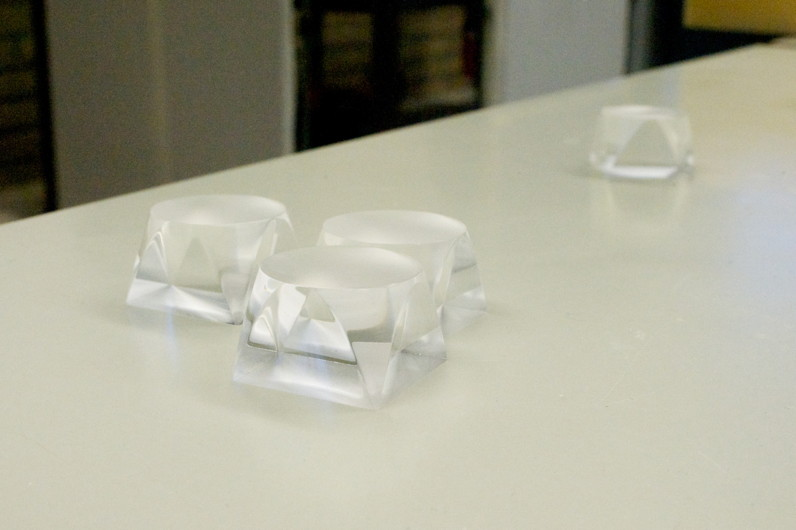
\includegraphics[width=0.47\linewidth]{blokjes}
    \label{fig:blokjes}
    \caption{De aansluitblokjes tussen de lichtgeleider en de \pmt.}
\end{figure}

\begin{figure}
    \centering
    \subfloat[]{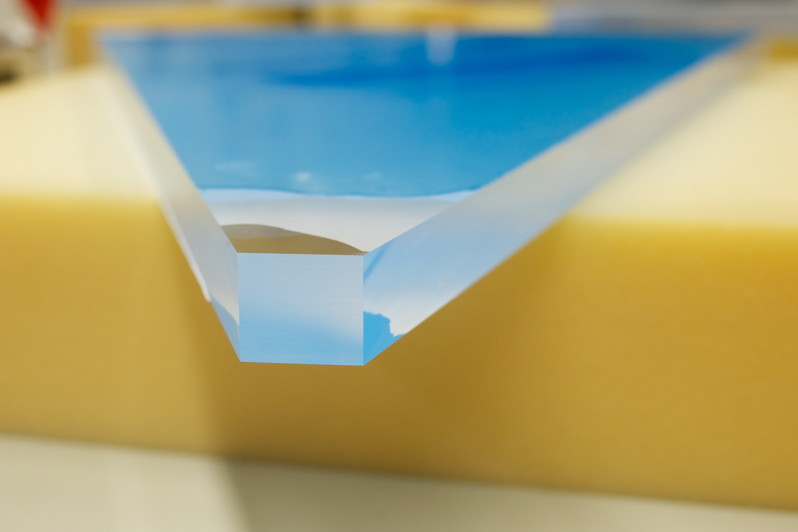
\includegraphics[width=0.47\linewidth]{lichtgeleider}
                \label{fig:lichtgeleider}}
    \subfloat[]{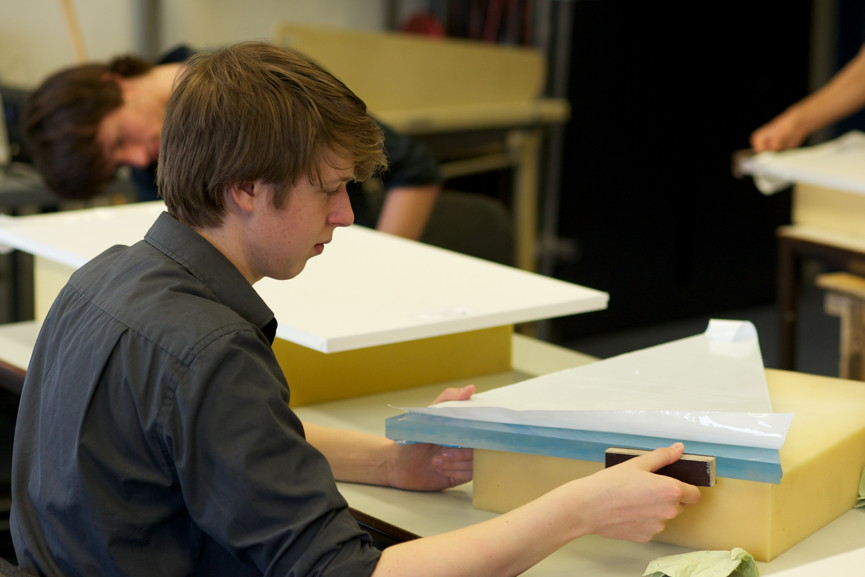
\includegraphics[width=0.47\linewidth]{schuren}
                \label{fig:schuren}}
    \caption{Het schuren van de lichtgeleiders en scintilatoren.}
\end{figure}

\begin{figure}
    \centering
    \subfloat[]{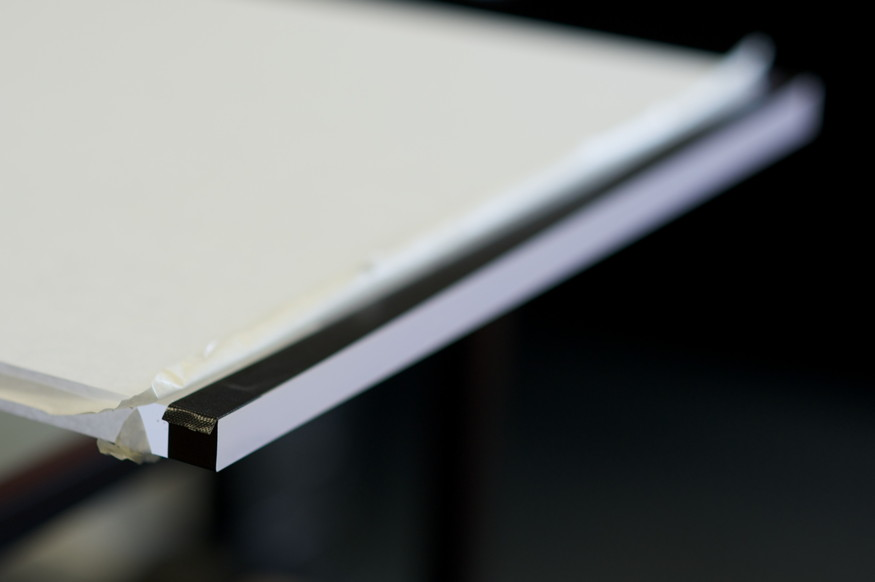
\includegraphics[width=0.47\linewidth]{rand_afplakken}
                \label{fig:rand_afplakken}}
    \subfloat[]{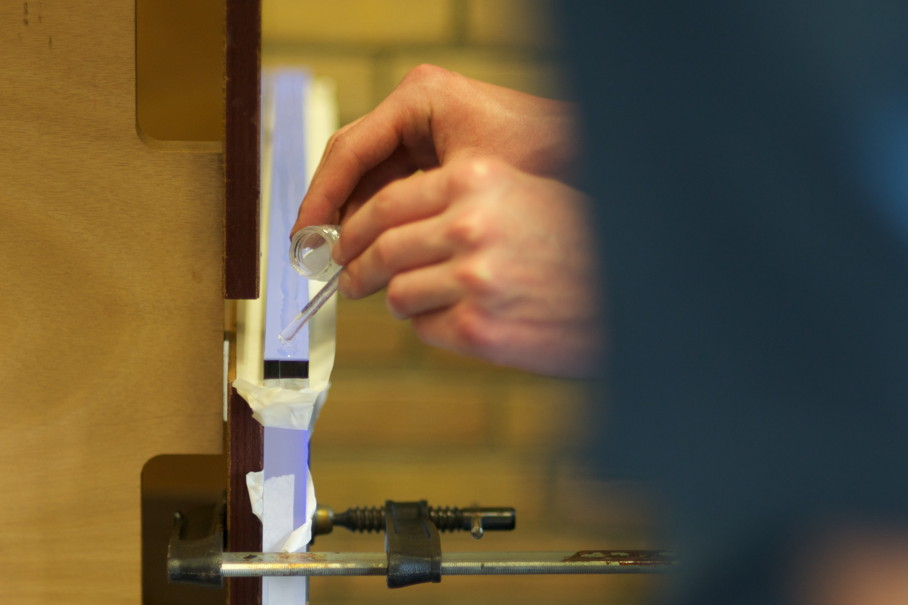
\includegraphics[width=0.47\linewidth]{lijmen}
                \label{fig:lijmen}}
    \caption{Het afplakken van de randen zodat er geen lijm op het
             materiaal komt waar het niet moet komen. En het aanbrengen
             van de lijm.}
\end{figure}

\begin{figure}
    \centering
    \subfloat[]{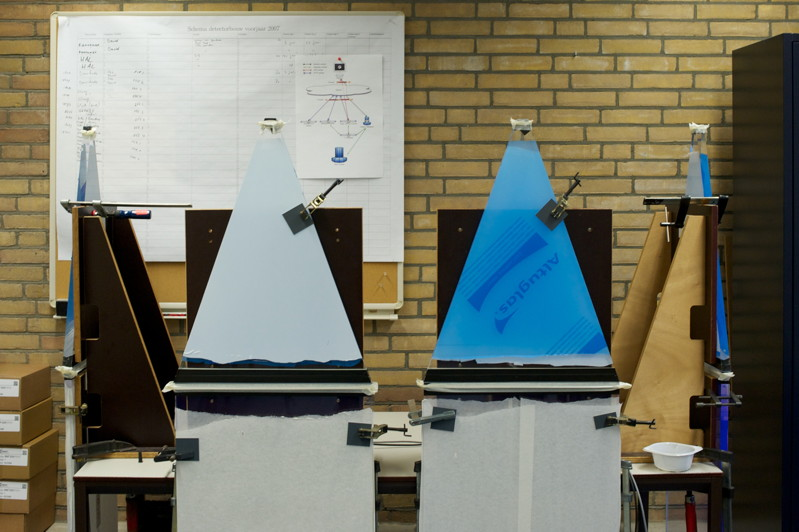
\includegraphics[width=0.47\linewidth]{mal}
                \label{fig:mal}}
    \subfloat[]{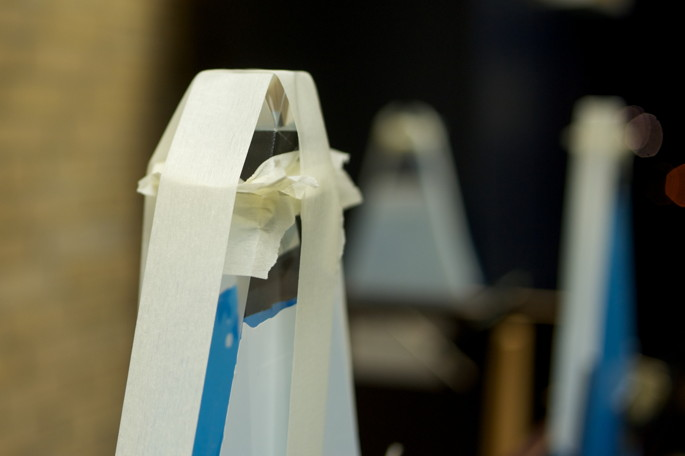
\includegraphics[width=0.47\linewidth]{blokje_verankering}
                \label{fig:blokje_verankering}}
    \caption{De gelijmde detector in de mal verankerd aan het drogen.}
\end{figure}

\begin{figure}
    \centering
    \subfloat[]{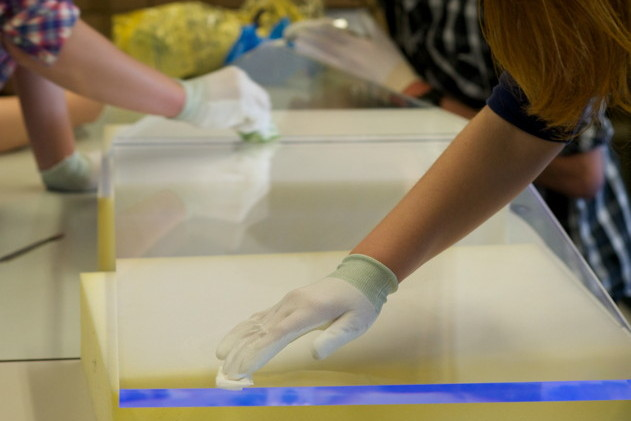
\includegraphics[width=0.47\linewidth]{poetsen_detector}
                \label{fig:poetsen_detector}}
    \subfloat[]{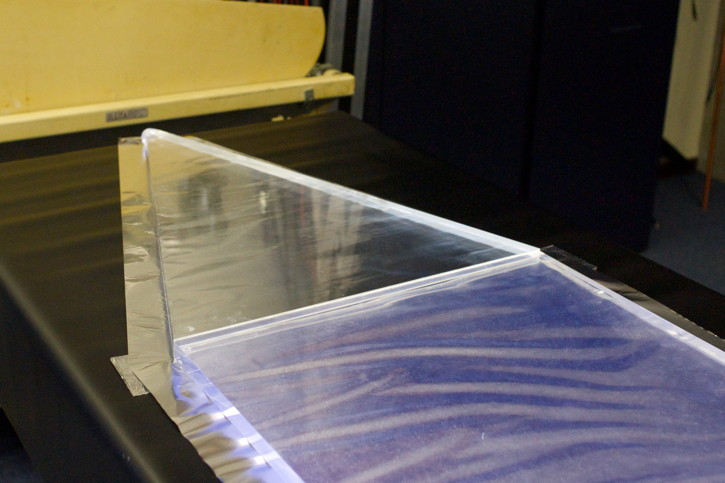
\includegraphics[width=0.47\linewidth]{open_detector}
                \label{fig:open_detector}}
    \caption{De detector goed met alcohol poetsen voor het plaatsen op
             het inpak folie.}
\end{figure}

\begin{figure}
    \centering
    \subfloat[]{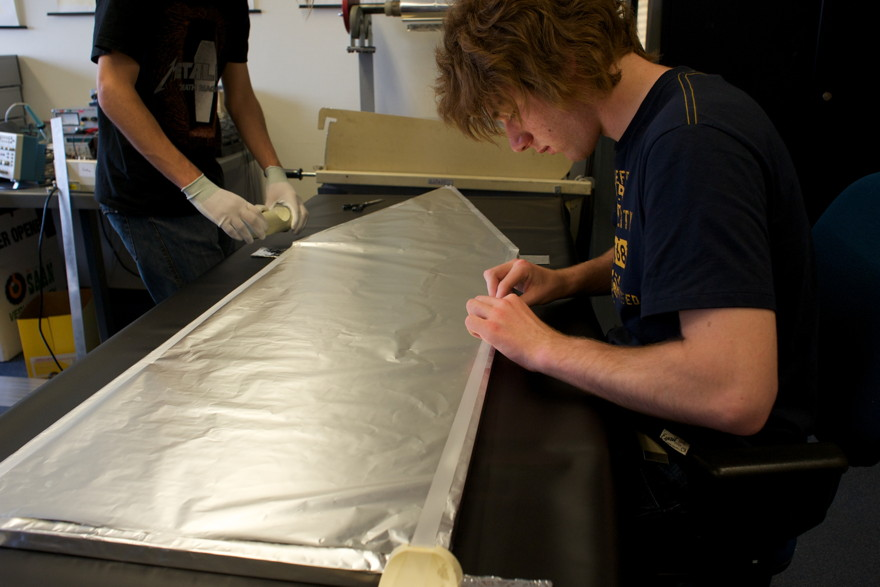
\includegraphics[width=0.47\linewidth]{aluminiumfolie_afplakken}
                \label{fig:aluminiumfolie_afplakken}}
    \subfloat[]{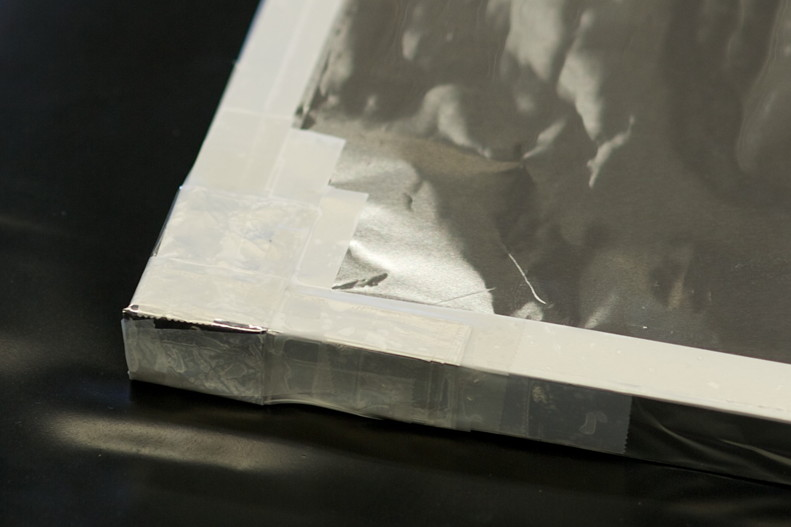
\includegraphics[width=0.47\linewidth]{hoek_versteviging}
                \label{fig:hoek_versteviging}}
    \caption{Inpakken van de detector. Verstevigde hoeken goed vast geplakt.}
\end{figure}

\begin{figure}
    \centering
    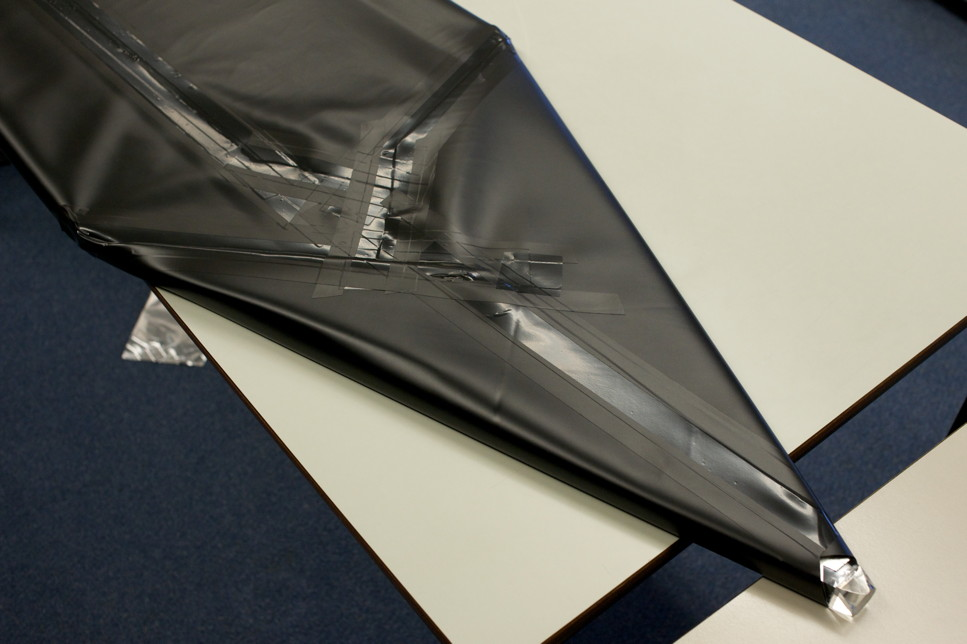
\includegraphics[width=0.47\linewidth]{vijverfolie_tape}
    \label{fig:vijverfolie_tape}
    \caption{De detector helemaal ingepakt, op \pmt na.}
\end{figure}

\begin{figure}
    \centering
    \subfloat[]{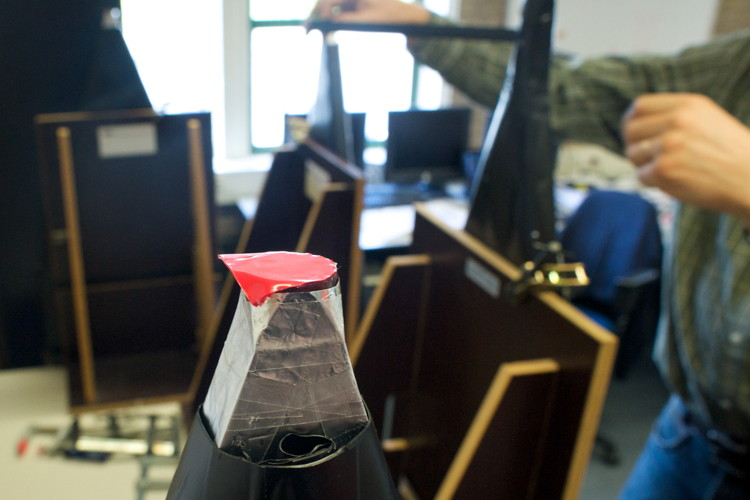
\includegraphics[width=0.47\linewidth]{optisch_tape}
                \label{fig:optisch_tape}}
    \subfloat[]{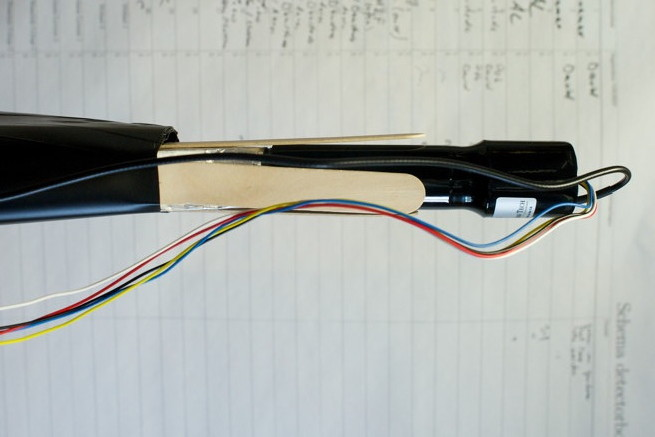
\includegraphics[width=0.47\linewidth]{pmt_spalken}
                \label{fig:pmt_spalken}}
    \caption{Optisch tape op het aansluitblokje en de \pmt bevestigd,
             met spalken ondersteund.}
\end{figure}


%\begin{thebibliography}{9}
%\end{thebibliography}

\end{document}
